\section{Diagramme de classe de conception}
\begin{figure}[H]
	\centering
	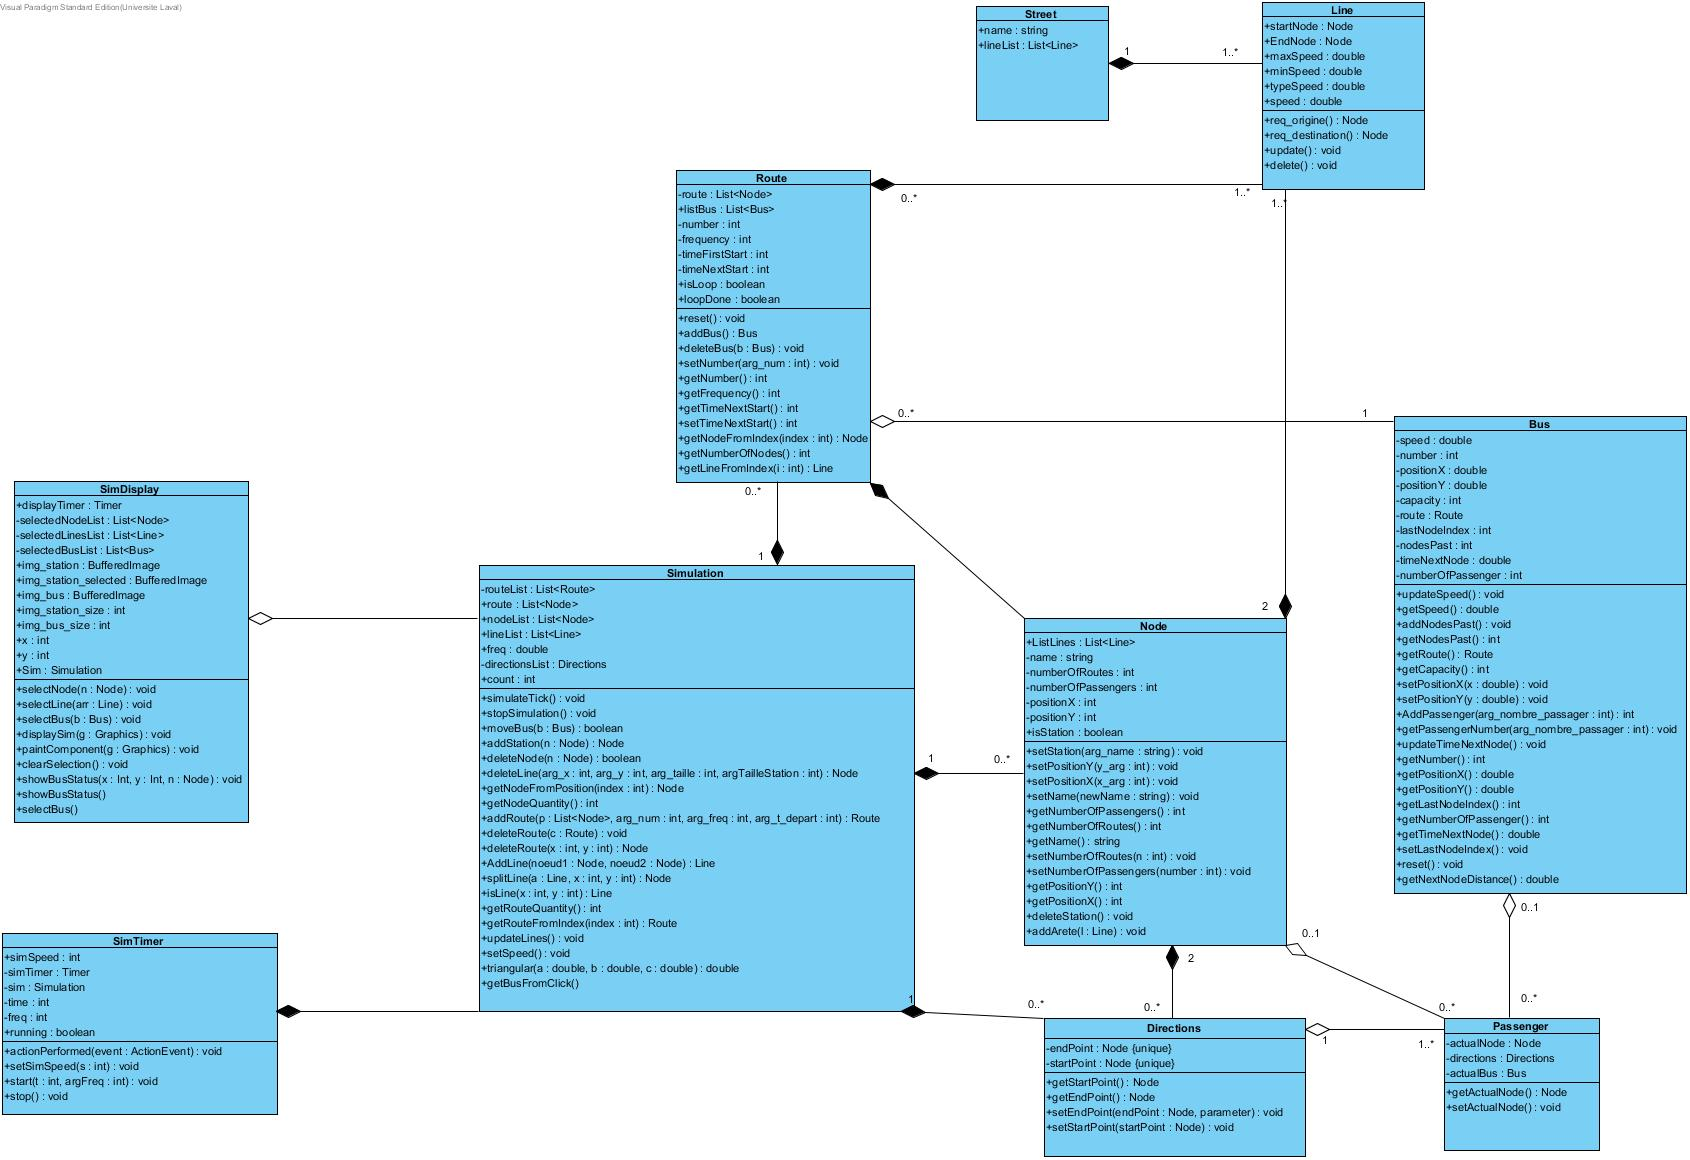
\includegraphics[scale=0.26]{fig/classDiagram.jpg}
	\caption{Diagramme de classe de conception de SimulatHEURE}
	\label{f:classDiag}
\end{figure}

Dans la figure \ref{f:classDiag}, on retrouve le diagramme de classes de conception. L'objet Simulation est le coeur de celui-ci et agit comme contr�leur. La classe SimDisplay permet quant � elle d'interagir avec l'utilisateur. Lorsqu'une simulation est cr��, il est possible de cr�er des noeuds (Node), des ar�tes (Line) des besoins en transport (Directions)  et des circuits (Route). Un passager quant � lui, poss�dera une position sur un noeud ou dans un Bus ainsi qu'un besoin en transport. Un circuit est compos� de noeuds et d'ar�te (Line) et poss�de des attributs repr�sentant la liste des noeuds, la liste des bus sur le circuit ainsi que la fr�quence par exemple. Plusieurs m�thodes sont impl�ment�s dans Route afin d'ajouter ou de retirer des bus et de retourner des informations comme le temps avant le prochain d�part. Dans la classe Line, les principaux attributs sont les noeuds de d�part et d'arriv� ainsi que diff�rents attributs permettant de quantifier la vitesse. Les m�thodes impl�ment�es dans cette classe permettent notamment de mettre � jour une Ar�te et de la supprimer. Ensuite, la classe Street est simplement un objet compos� de plusieurs ar�tes et contient donc comme attributs une liste d'ar�te ainsi qu'un nom de rue. L'objet Noeud, pouvant �tre cr�� � partir de Simulation, contient une liste d'ar�tes associ�es, un nom, une position spatiale ainsi que le nombre de circuits et de passagers qui y sont rattach�s. De plus, un objet a l'attribut isStation qui permet de d�terminer si ce noeud est une station. Les m�thodes rattach�es � Noeud permettent notamment d'y rattacher d'autres ar�tes ainsi que de d�placer le noeud dans l'espace. La classe Bus, elle, poss�de des attributs de position dans l'espace ainsi que diff�rentes informations comme la vitesse, le dernier noeud parcouru, le nombre de passagers, le circuit actuel et sa capacit�. Les m�thodes de cette classe permettent de mettre � jour la vitesse, le temps et la distance avant le prochain noeud. On peut �galement modifier le nombre de passagers et retourner l'index du dernier noeud parcouru dans son parcours. La classe SimTimer, dicte le rythme de la simulation et permet de contr�ler la vitesse, le d�part et l'arr�t de la simulation.

